\documentclass[a4paper, 12pt]{article}
\usepackage[utf8]{inputenc}
\usepackage[german]{babel}
\usepackage{hyperref}
\usepackage{graphicx}
\usepackage{titling}
\usepackage{array}

\title{Semantic Web-Anwendung zur Analyse von Bevölkerungsdaten in deutschen Städten}
\author{Lukas Ruminski, Nived Stephen und Sarah Kiki}
\date{\today}

\begin{document}

\begin{titlepage}
    \maketitle
    \begin{center}
        \Large\href{https://gitlab.imn.htwk-leipzig.de/semantic-web-migration/migration-backend}{gitlab.imn.htwk-leipzig.de/semantic-web-migration}
        \vfill
        \Large\ HTWK Leipzig - Semantic Web
    \end{center}
\end{titlepage}

\begin{titlepage}
    \tableofcontents % Add table of contents
\end{titlepage}

\section{Einleitung}
Die vorliegende Forschungsarbeit widmet sich der Entwicklung und Umsetzung einer innovativen Semantic Web-Anwendung zur tiefgreifenden Analyse von Bevölkerungsdaten in verschiedenen Städten Deutschlands. Im Fokus steht die Verknüpfung von semantischer Modellierung und Datenanalyse, um Einblicke in die Bevölkerungsstruktur, Migrationstrends und demografische Veränderungen auf höchst präzise und bedeutungsvolle Weise zu gewinnen.

\subsection{Hintergrund}
Die zunehmende Verfügbarkeit großer Mengen an Bevölkerungsdaten eröffnet die Möglichkeit, relevante Erkenntnisse über soziale, wirtschaftliche und demografische Phänomene zu gewinnen. Allerdings erfordert die Interpretation solcher Daten eine robuste Methodik, die über herkömmliche statistische Ansätze hinausgeht. Das Semantic Web bietet hierbei eine vielversprechende Lösung, indem es strukturierte, vernetzte und semantisch angereicherte Datenmodelle ermöglicht.

\subsection{Zielsetzung}
Das Hauptziel dieser Forschungsarbeit besteht darin, die Synergie zwischen dem Semantic Web und der Analyse von Bevölkerungsdaten zu nutzen, um tiefgreifende Einblicke in das Verhalten, die Verteilung und die Veränderungen der Bevölkerung in verschiedenen deutschen Städten zu erhalten.\\
Durch die Entwicklung einer spezialisierten Ontologie und die Verknüpfung von Bevölkerungsdaten in einem semantischen Kontext streben wir danach, Fragen von sozialer und demografischer Bedeutung zu beantworten und bisher unentdeckte Zusammenhänge aufzudecken.

\subsection{Methodik}
Die Forschungsarbeit gliedert sich in mehrere Schritte:
\begin{enumerate}
    \item Datenerfassung und Modellierung: \\
    Bevölkerungsdaten von verschiedenen deutschen Städten, einschließlich Informationen zu Ausländern, Schutzsuchenden, Altersgruppen und Aufenthaltsdauern, werden erfasst und in einer eigens entwickelten Ontologie modelliert.
    \item Tripelgenerierung und semantische Anreicherung: \\
    Basierend auf der Ontologie werden Bevölkerungsdaten in Tripel umgewandelt und semantisch angereichert, um Beziehungen zwischen den Datenpunkten herzustellen.
    \item Integration in Graph Datenbank: \\
    Die semantisch angereicherten Daten werden in eine Graph Datenbank hochgeladen, um eine effiziente Speicherung, Abfrage und Verknüpfung der Daten zu ermöglichen.
    \item SPARQL-basierte Analyse: \\
    Mithilfe von SPARQL-Abfragen werden gezielte Fragestellungen beantwortet, um Erkenntnisse über Bevölkerungsstruktur, Migrationstrends und demografische Veränderungen zu gewinnen.
\end{enumerate}

\section{Relevante Datenquellen}
Wir haben nur vollständige Datenquellen für das Jahr 2022 gefunden. Mit der Wayback Machine war es uns möglich, auch Daten für das Jahr 2021 zu erhalten. Deshalb haben wir uns nur auf diese Jahre fokussiert.

\subsection{Bevölkerung insgesamt und Ausländeranteil}
Die Daten stammen vom Statistischen Bundesamt (Destatis) und wurden bis zum 31. Dezember 2021 fortgeschrieben. Diese Daten sind auf den offiziellen Websites \href{www.destatis.de}{www.destatis.de} und \href{www.statistik-portal.de}{www.statistik-portal.de} verfügbar.

\subsection{Ausländische Bevölkerung}
Die Daten wurden zum 31. Dezember 2022 im Ausländerzentralregister \linebreak (AZR) erfasst und sind ebenfalls auf \href{www.destatis.de}{www.destatis.de} zu finden.

\subsection{Schutzsuchende}
Die Daten wurden ebenfalls bis zum 31. Dezember 2022 im Ausländerzentral-\linebreak register (AZR) erfasst. Informationen über registrierte Schutz-\linebreak suchende können aus der GENESIS-Online-Datenbank des Statistischen Bundesamts gewonnen werden. Die Daten sind in Form von Tabellen im XLSX-, XLS-, CSV- und HTML-Format herunterladbar. Zudem bietet das Statistische Bundesamt die Möglichkeit, die Daten in Diagrammen, interaktiven Karten anzuzeigen und eine API-Programmierschnittstelle zur automatisierten Datenverarbeitung zu nutzen.


\subsection{MediaWiki Action API}
Um detaillierte Informationen über einzelne Städte zu erhalten, haben wir die \href{https://www.mediawiki.org/wiki/API:Main_page}{MediaWiki-API} genutzt, um Links zu den individuellen Städteseiten zu generieren. Diese Links ermöglichen den direkten Zugriff auf umfassende Informationen über jede Stadt, einschließlich Bevölkerungsstatistiken, geografischer Merkmale und kultureller Aspekte. Die Verwendung der MediaWiki-API hat es uns ermöglicht, gezielte Daten für verschiedene Städte abzurufen und eine umfassendere Analyse der regionalen Unterschiede und Entwicklungen vorzunehmen.

\section{Ontologie}
Unsere Ontologie sollte den demografischen Wandel in Deutschland darstellen. Um die Ontologie zu erstellen, haben wir die Methode nach Grüninger und Fox genutzt. Um die richtigen Klassen und Eigenschaften zu bestimmen, haben wir Kompetenzfragen entwickelt, die mithilfe der Ontologie beantwortet werden können. Wir haben den WebVOWL Editor erfolgreich genutzt, um unsere Ontologie zu erstellen. Diese Plattform bietet eine interaktive Web-Benutzeroberfläche, die es uns ermöglicht, die Ontologie einfach und visuell ansprechend zu entwickeln. Die intuitive Schnittstelle erlaubt es uns, komplexe Beziehungen und Konzepte leicht zu gestalten und Änderungen in Echtzeit zu visualisieren. Dies erleichtert den Entwicklungsprozess und führt zu einer klareren Repräsentation unserer Daten und Strukturen.
\newline \newline

\subsection{Vokabular}
\subsubsection{Präfixe}
Die Präfixe, die für die Ontologie verwendet werden, sind: \\ \\
\texttt{mo:         <https://gitlab.imn.htwk-leipzig.de/semantic-web-migration/\\ migration-backend/-/blob/main/Ontology/migrationOntology.ttl\#> . }\\
\texttt{rdf:        <http://www.w3.org/1999/02/22-rdf-syntax-ns\#> .  }\\
\texttt{rdfs: 		<http://www.w3.org/2000/01/rdf-schema\#> .  }\\
\texttt{owl: 		<http://www.w3.org/2002/07/owl\#> .  }\\
\texttt{xsd: 		<http://www.w3.org/2001/XMLSchema\#> .  }\\
\texttt{dc: 		<http://purl.org/dc/elements/1.1/\#> .  }\\


\subsubsection{Klassendefinitionen (Class Definitions)}

In diesem Abschnitt werden verschiedene OWL-Klassen definiert, die im Ontologie-Modell verwendet werden. Jede Klasse repräsentiert einen bestimmten Konzepttyp wie Stadt, Bevölkerung oder Ausländer. Diese Klassen dienen als Grundbausteine für die Modellierung von Beziehungen und Eigenschaften. \\

\begin{tabular}{|l|l|l|l|l|}
    \hline
    rdfs:label & rdf:type \\
    \hline
    City & owl:Class  \\
    Population & owl:Class  \\
    Foreigners & owl:Class  \\
    Germans & owl:Class  \\
    ProtectionSeekers & owl:Class  \\
    Agegroup & owl:Class  \\
    Duration\_of\_stay & owl:Class  \\
    Residence\_Status & owl:Class  \\
    \hline
\end{tabular}

\subsubsection{Objekteigenschaften (Object Properties)}

Hier werden die Beziehungen zwischen den OWL-Klassen durch Objekteigenschaften beschrieben. Diese Eigenschaften definieren, wie verschiedene Klassen miteinander in Beziehung stehen. Beispielsweise wird die Beziehung zwischen Stadt und Bevölkerung durch die Eigenschaft hatBevölkerung definiert, die angibt, welche Bevölkerung in welcher Stadt lebt. \\

\begin{tabular}{|l|l|l|l|l|}
    \hline
    rdfs:label & rdf:type & rdfs:domain & rdfs:range \\
    \hline
    
    hasPopulation & owl:ObjectProperty & City & Population \\
    hasForeigners & owl:ObjectProperty & Population & Foreigners \\
    hasGermans & owl:ObjectProperty & Population & Germans \\
    PopulationAgegroup & owl:ObjectProperty & Population & Agegroup \\
    ForeignersAgegroup & owl:ObjectProperty & Foreigners & Agegroup \\
    GermanAgegroup & owl:ObjectProperty & Germans & Agegroup \\
    hasDurationOfStay & owl:ObjectProperty & Foreigners & Duration\_of\_stay \\
    hasResidenceStatus & owl:ObjectProperty & Foreigners & Residence\_Status \\
    hasProtectionSeekers & owl:ObjectProperty & Population & ProtectionSeekers \\
    \hline
\end{tabular}

\subsubsection{Datentyp-Eigenschaften (Datatype Properties)}

Dieser Abschnitt behandelt Eigenschaften, die konkrete Datenwerte speichern, wie z.B. den Namen einer Stadt, das Jahr ihrer Gründung oder die Gesamtbevölkerung. Diese Eigenschaften sind mit bestimmten Klassen und Datentypen verknüpft, um die Informationen in der Ontologie genau zu definieren. \\

\begin{tabular}{|l|l|l|l|l|}
    \hline
    rdfs:label & rdfs:domain & rdfs:range \\
    \hline

    name & City & xsd:integer \\
    year & City & xsd:integer \\
    wikiLink & City & xsd:integer \\
    regional\_code & City & xsd:integer \\

    totalPopulation & Population & xsd:integer \\
    totalForeigners & Foreigners & xsd:integer \\
    fromEU & Foreigners & xsd:integer \\
    from\_non\_EU & Foreigners & xsd:integer \\
    totalGermans & Germans & xsd:integer \\
    
    with\_temporary\_residence\_permit & Residence\_Status & xsd:integer \\
    with\_permanent\_residence\_permit & Residence\_Status & xsd:integer \\
    with\_permission\_to\_remain & Residence\_Status & xsd:integer \\
    with\_permission\_to\_remain\_untill\_deported & Residence\_Status & xsd:integer \\
    with\_EU\_residence\_permit & Residence\_Status & xsd:integer \\

    recognized & ProtectionSeekers & xsd:integer \\
    cancelled & ProtectionSeekers & xsd:integer \\
    open & ProtectionSeekers & xsd:integer \\
    
    under2years & Duration\_of\_stay & xsd:integer \\
    2to10years & Duration\_of\_stay & xsd:integer \\
    from10to25years & Duration\_of\_stay & xsd:integer \\
    from\_25\_years\_and\_more & Duration\_of\_stay & xsd:integer \\
    
    
    under\_6\_years & Agegroup & xsd:integer \\
    between\_6\_and\_15\_years & Agegroup & xsd:integer \\
    between\_15\_and\_65\_years & Agegroup & xsd:integer \\
    older\_than\_65\_years & Agegroup & xsd:integer \\
    
    \hline
\end{tabular}

\subsubsection{Ontologie (Graphisch)}
Alle für die Ontologie erforderlichen Dateien befinden sich im Ordner Ontologie in unserem Repository
\newline
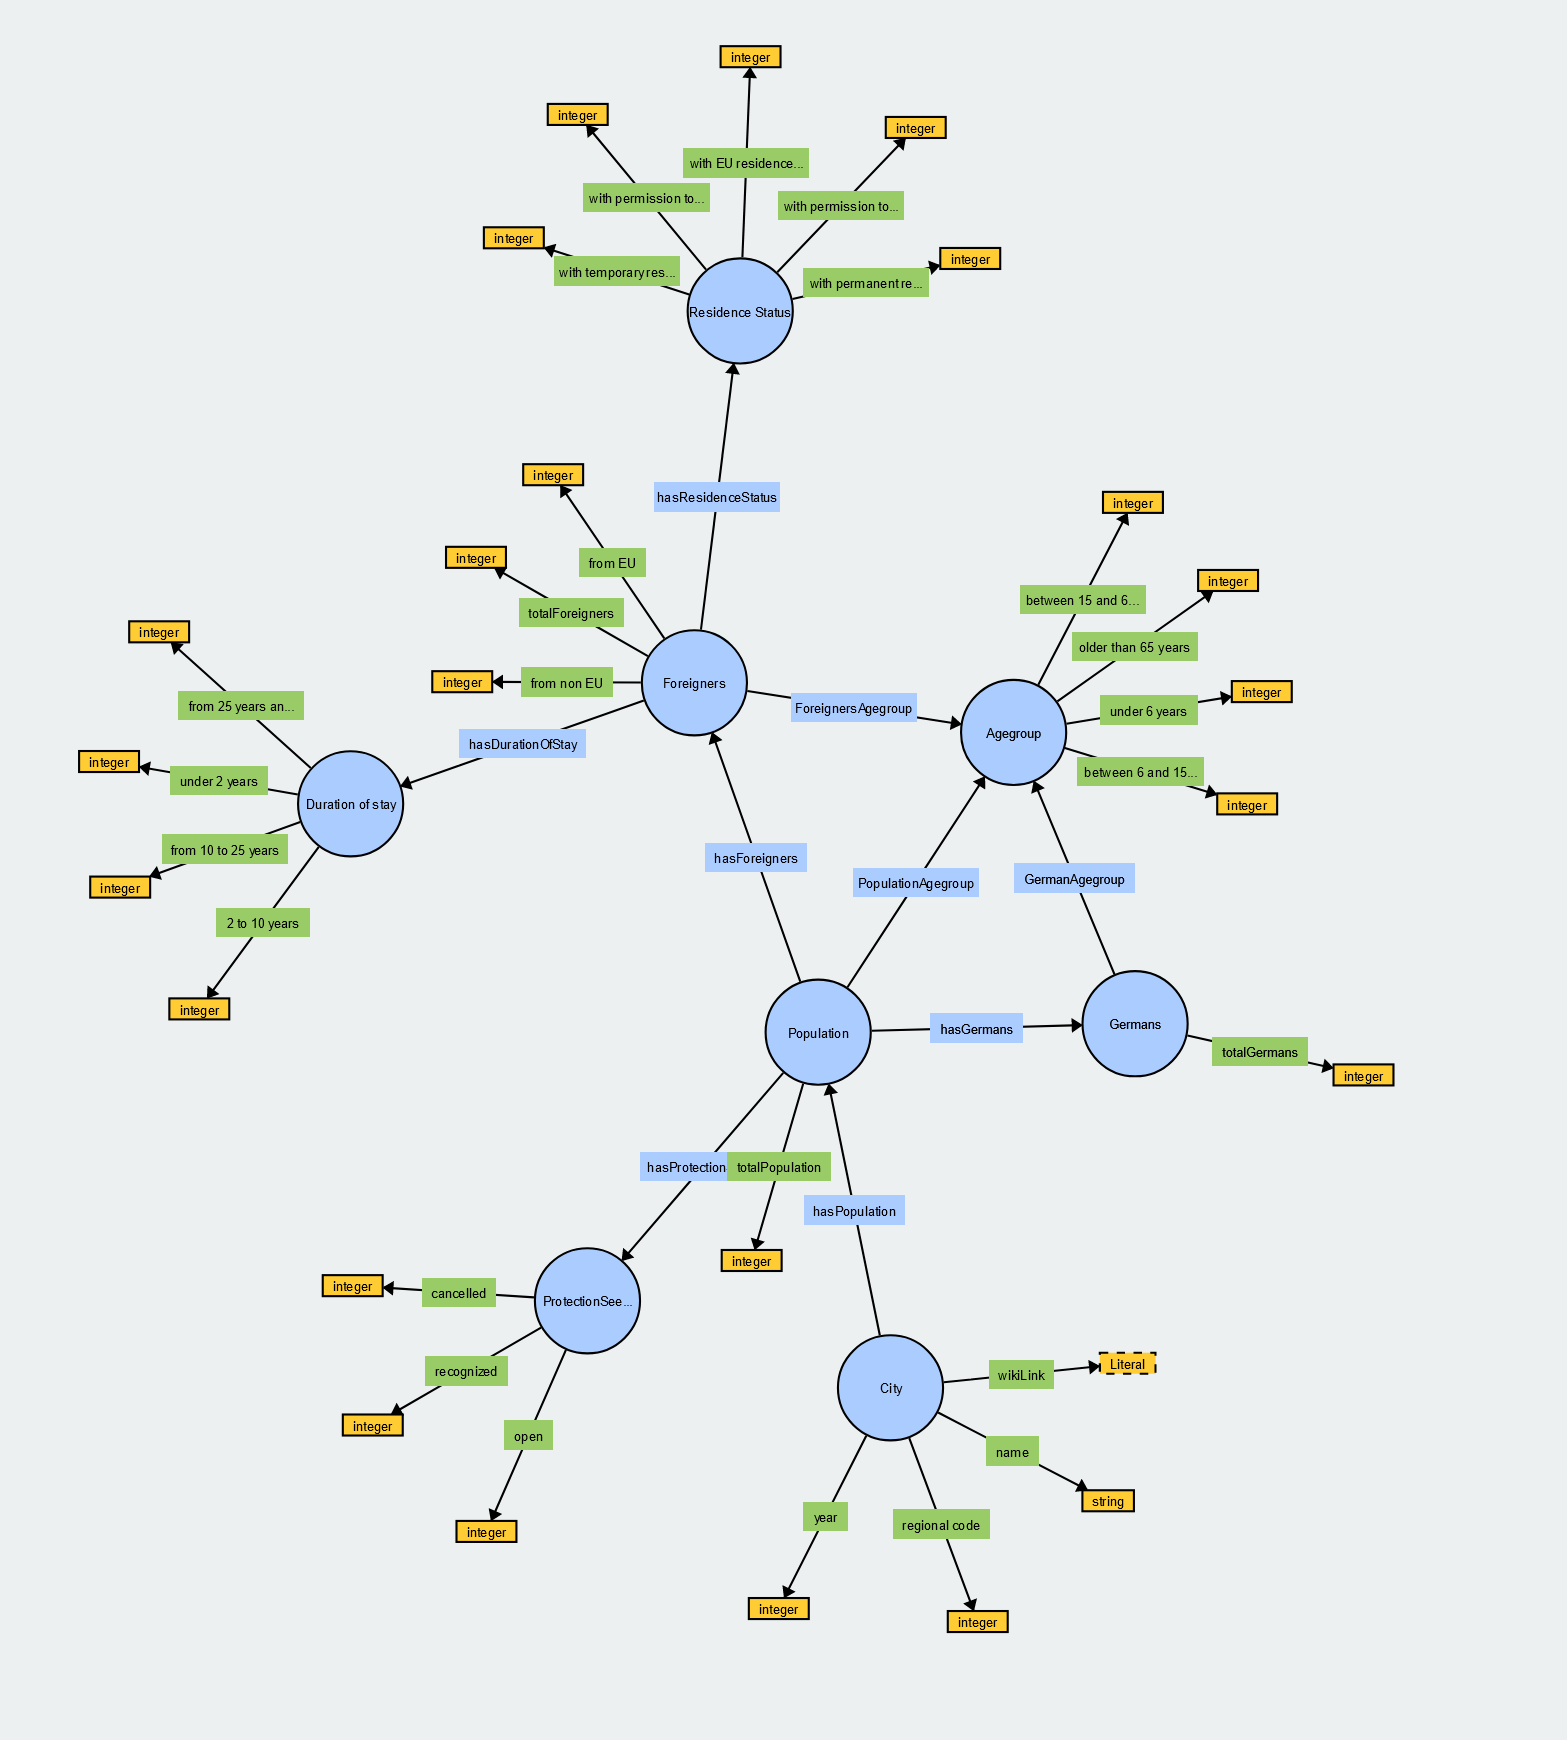
\includegraphics[width=\textwidth]{migration.png}
\newline \newline

\section{Extraktion und Aufbereitung relevanter Daten}
Die vorliegenden Daten wurden zunächst aus einer CSV-Datei extrahiert und anschließend in das JSON-Format umgewandelt. Diese Umwandlung erfolgte, um einen verbesserten Zugriff und eine flexiblere Verarbeitung der Daten zu ermöglichen. Die umgewandelten JSON-Daten bildeten die Grundlage für die nächste Entwicklungsphase. Hierbei wurde ein speziell entwickeltes TypeScript-Programm erstellt, das sich als äußerst leistungsfähig erwiesen hat. Das Programm ist in der Lage, die JSON-Daten zu lesen und gezielt darauf zuzugreifen. Dieser Zugriff bildet die Grundlage für die darauf folgende Datenverarbeitung.

In einem weiteren Schritt wurde die Funktionalität implementiert, um die JSON-Daten in sogenannte Tripel zu transformieren. Diese Transformation war entscheidend, um semantische Beziehungen und Zusammenhänge zwischen den Datenpunkten herzustellen. Dabei kam eine vordefinierte Ontologie zum Einsatz, die es ermöglichte, die Daten in ein strukturiertes und aussagekräftiges Format zu bringen.

Die generierten Tripel bilden die Grundlage für die Erstellung von Turtle-Dateien. Hierbei wurden nicht nur die eigentlichen Daten einbezogen, sondern auch Namensräume, die die semantische Bedeutung der Datenpunkte verdeutlichen. Die Turtle-Dateien stellen somit eine hochwertige und umfassende Darstellung der Daten dar, die sich ideal für weitere Analysen und Interpretationen eignet.

Die Quellcodedateien in TypeScript zur Realisierung dieser Prozesskette sind verfügbar und befinden sich im übersichtlichen "src"-Ordner. Die Kompilierung der TypeScript-Dateien erfolgt mit dem Befehl \texttt{tsc}. Die Ausführung des Befehls \texttt{node tripleGenerator.js > data2022.ttl} führt zur Generierung der Turtle-Dateien, die die Daten in einer für Menschen lesbaren und maschinenverarbeitbaren Form präsentieren. Die generierten Tripel-Daten werden im Ordner RDF Triples in unserem GitLab-Repository gespeichert.

\section{SPARQL-Anfrage}
Unsere Turtle Dateien wurden erfolgreich in GraphDB hochgeladen. Dadurch können wir gezielte SPARQL-Abfragen auf Grundlage dieser Daten durchführen. Dies ermöglicht uns, spezifische Informationen zu unseren Kompetenzfragen zu extrahieren und zu analysieren. Die Interaktivität von \linebreak GraphDB ermöglicht es uns, die Abfragen direkt zu testen und relevante Ergebnisse zu erhalten.

\subsection{Kompetenzfragen und Ergebnisse}
Die Kompetenzfragen, zusammen mit den dazugehörigen SPARQL-Abfragen und den erzielten Ergebnissen, sind wie folgt formuliert:

\begin{enumerate}
    \item Wie viele Ausländer leben in Leipzig? \\ \\
    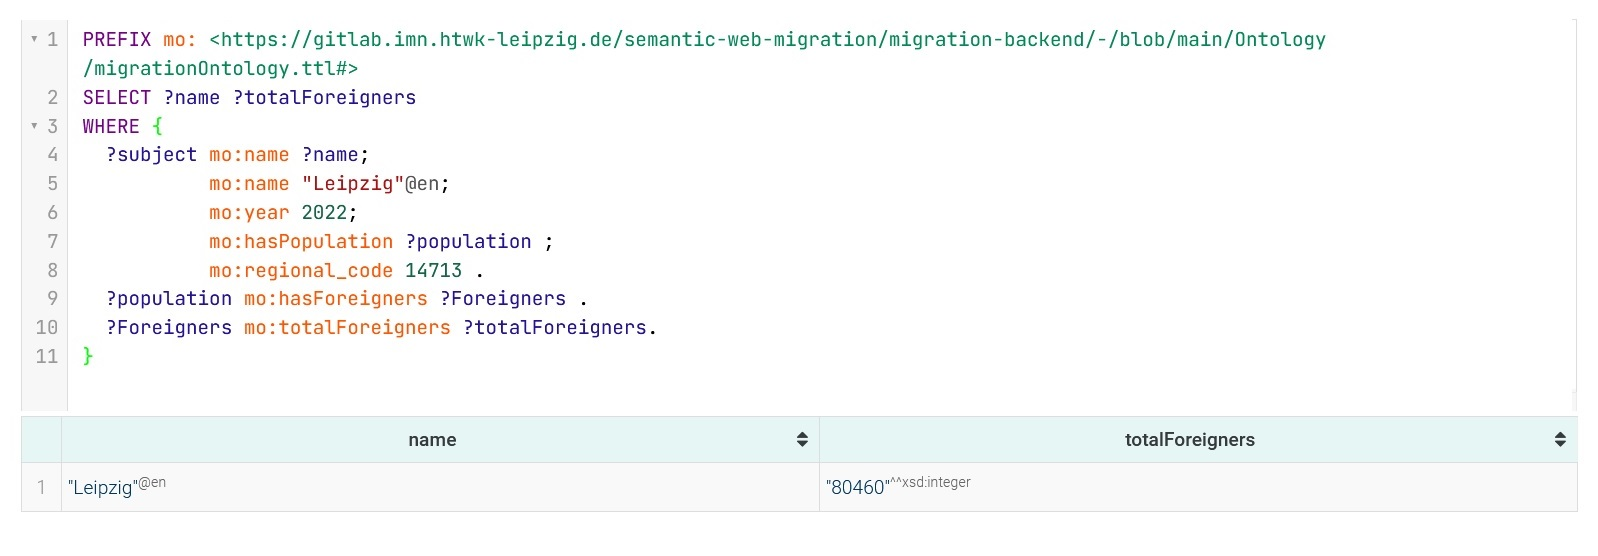
\includegraphics[width=1\textwidth]{Frage1.jpg} \\
    \item Wie viele Ausländer in Hamburg sind älter als 65 Jahre? \\ \\
    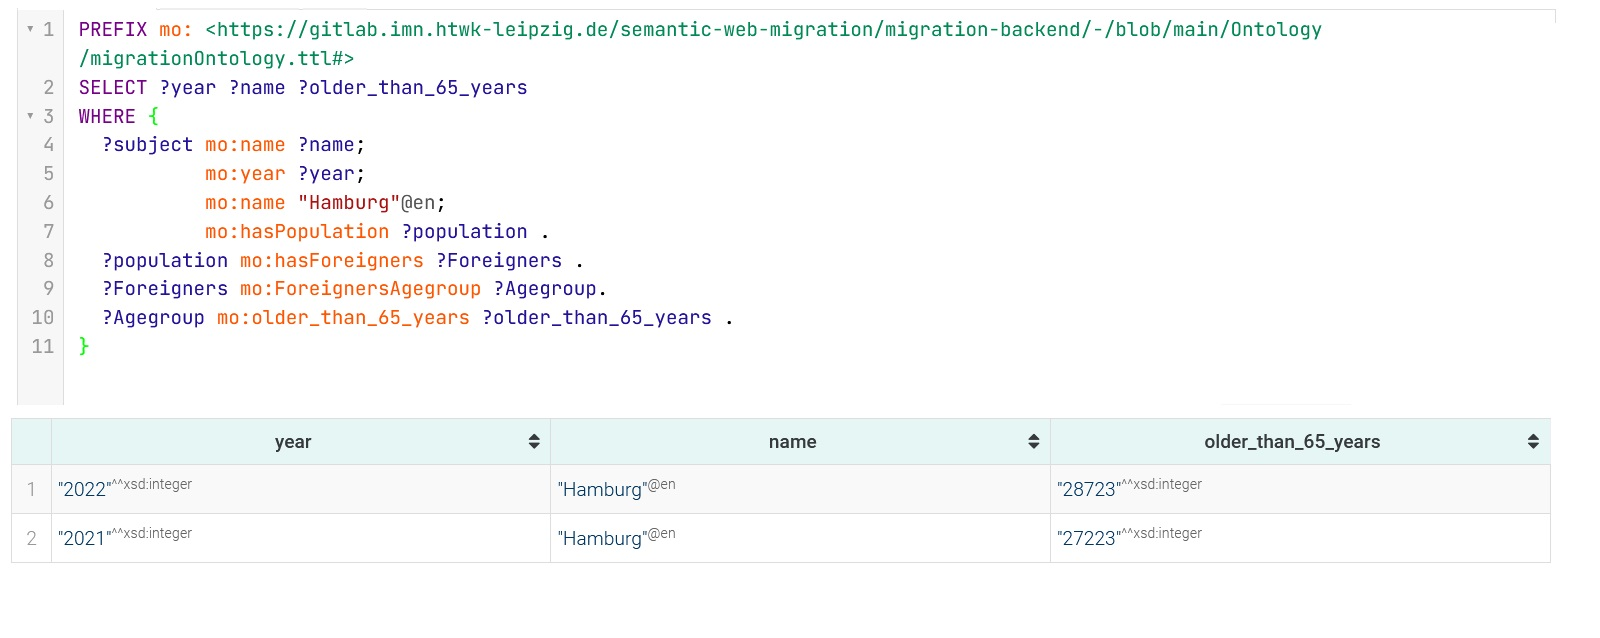
\includegraphics[width=1\textwidth]{Frage2.jpg} \\
    \item Was ist die Wikiseite von Leipzig? \\ \\
    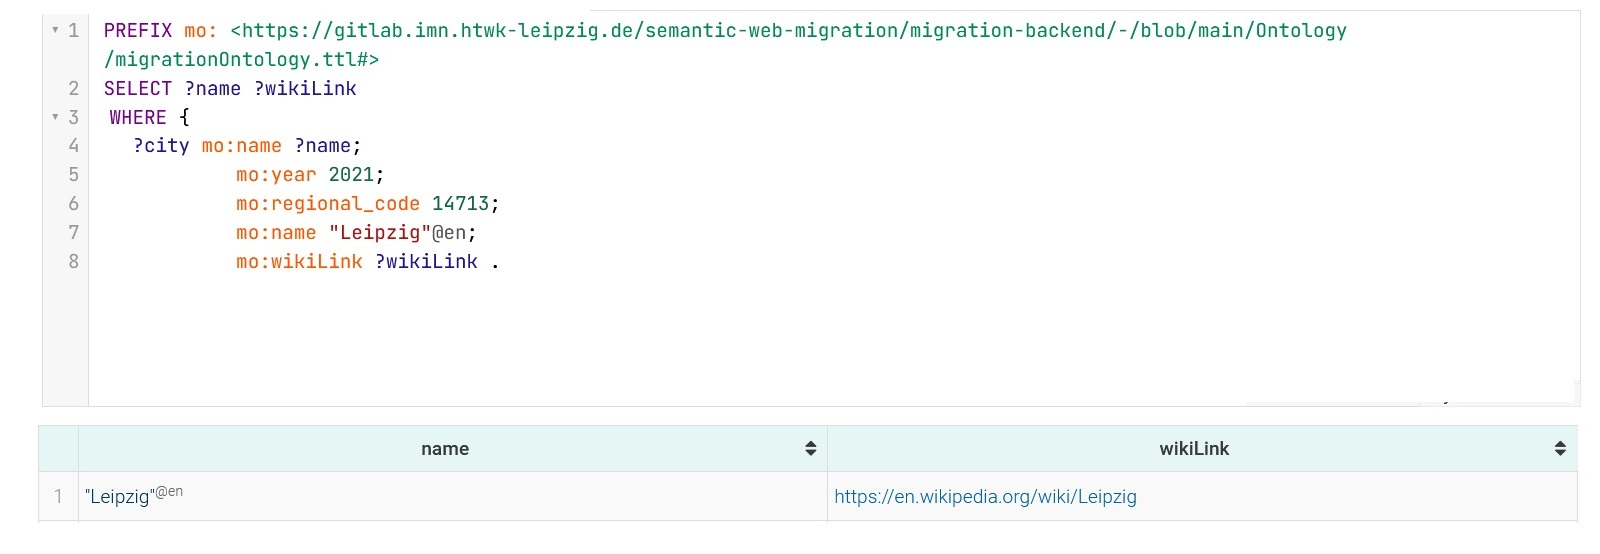
\includegraphics[width=1\textwidth]{Frage3.jpg} \\
    \item Wie viele Asylsuchende gibt es in Deutschland? \\ \\
    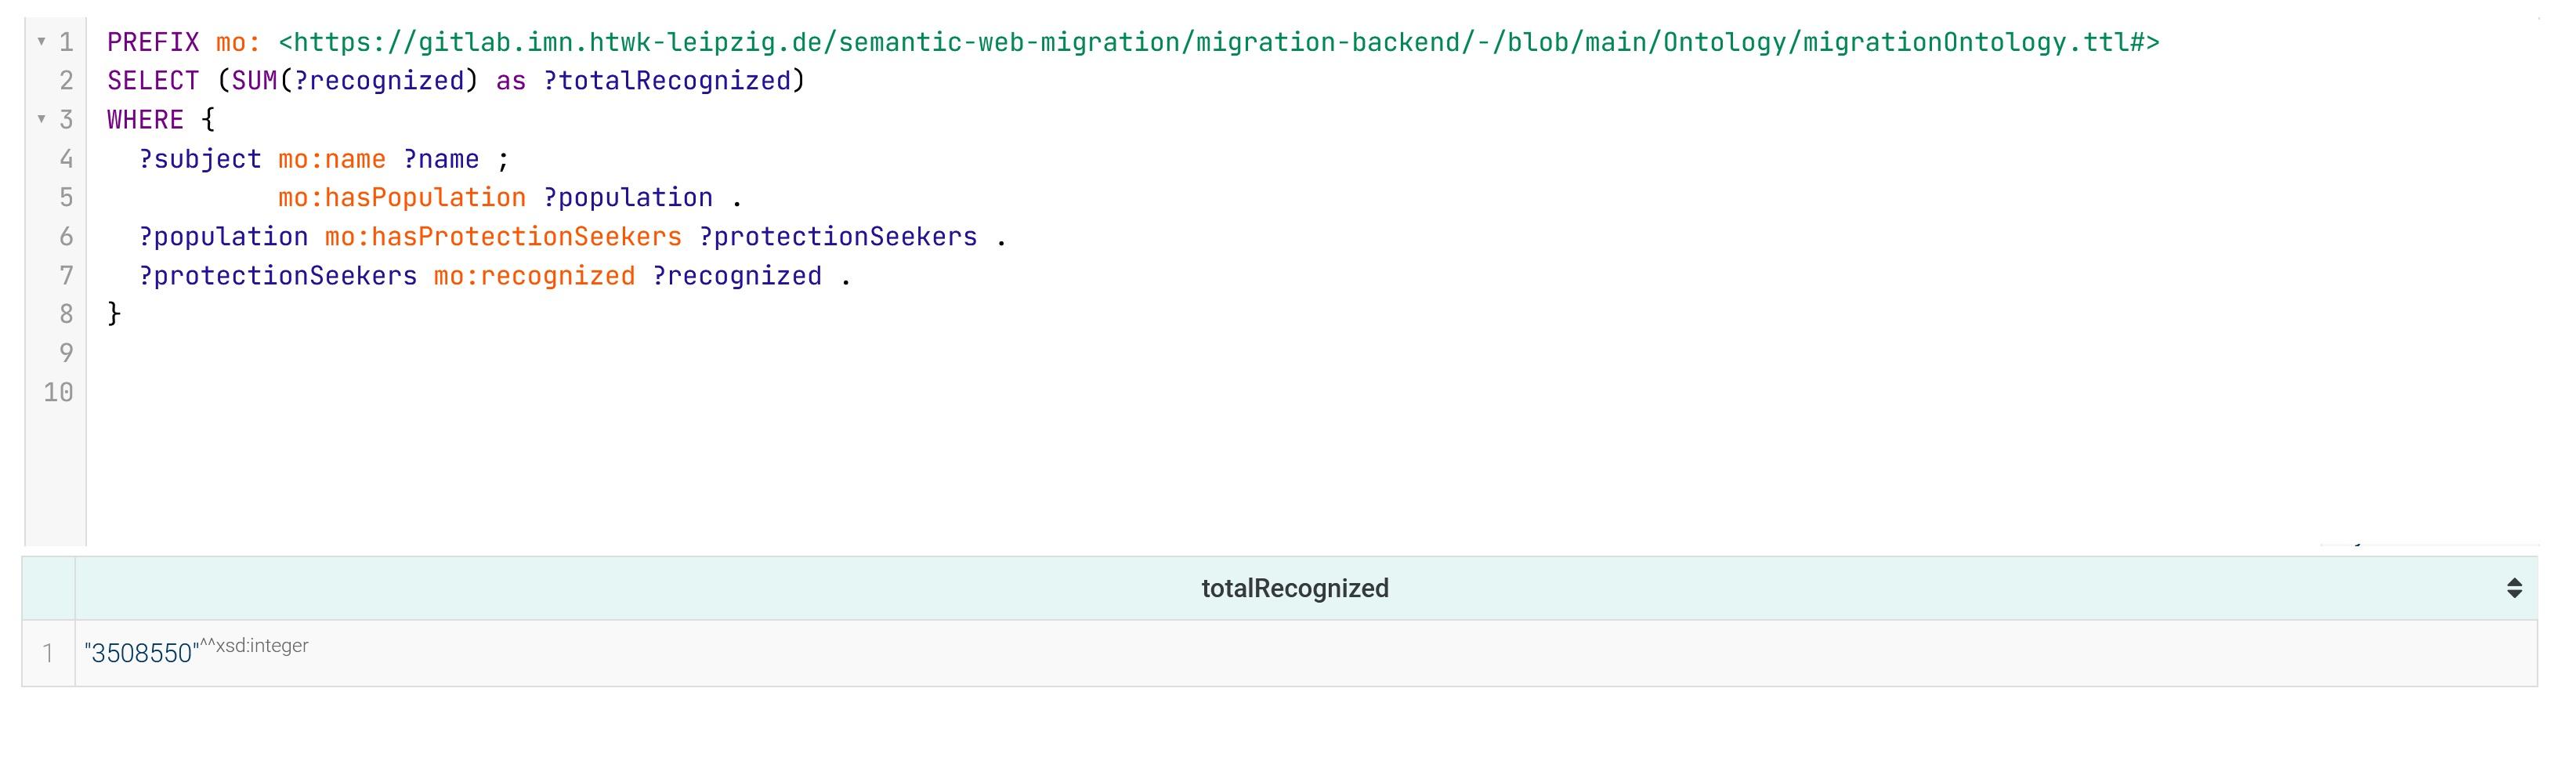
\includegraphics[width=1\textwidth]{Frage4.jpg} \\
    \item Wie viele Ausländer leben in Frankfurt schon länger als 25 Jahre? \\ \\
    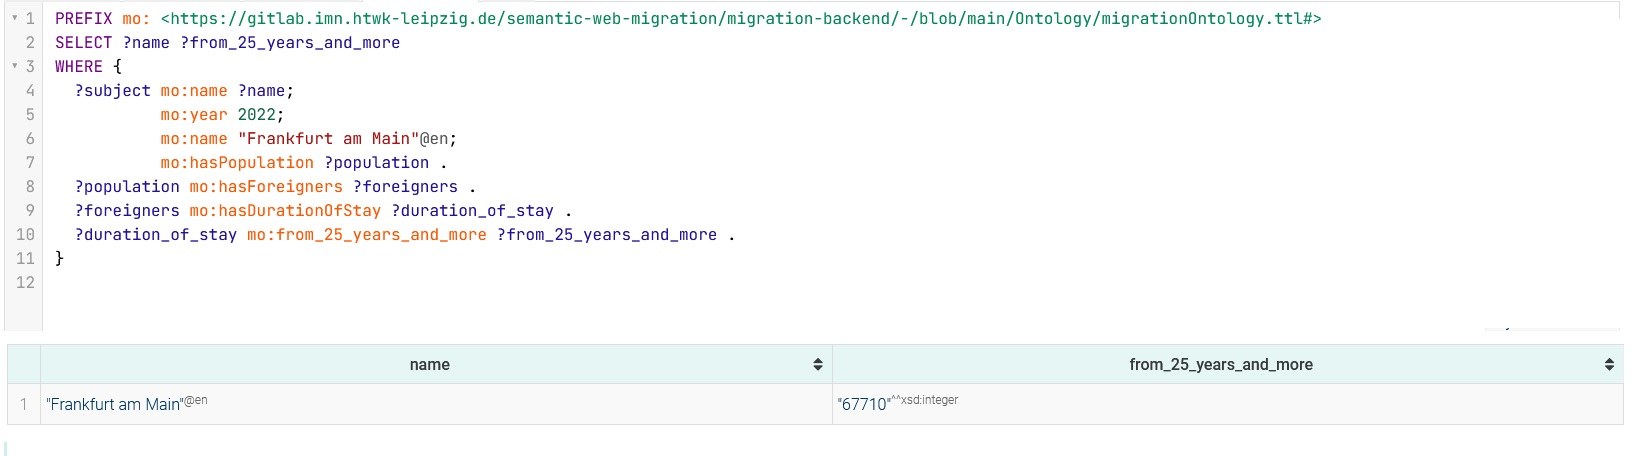
\includegraphics[width=1\textwidth]{Frage5.jpg} \\
    \item Wie hat sich die Anzahl der Ausländer zwischen 2021 und 2022 in Leipzig verändert? \\ \\
    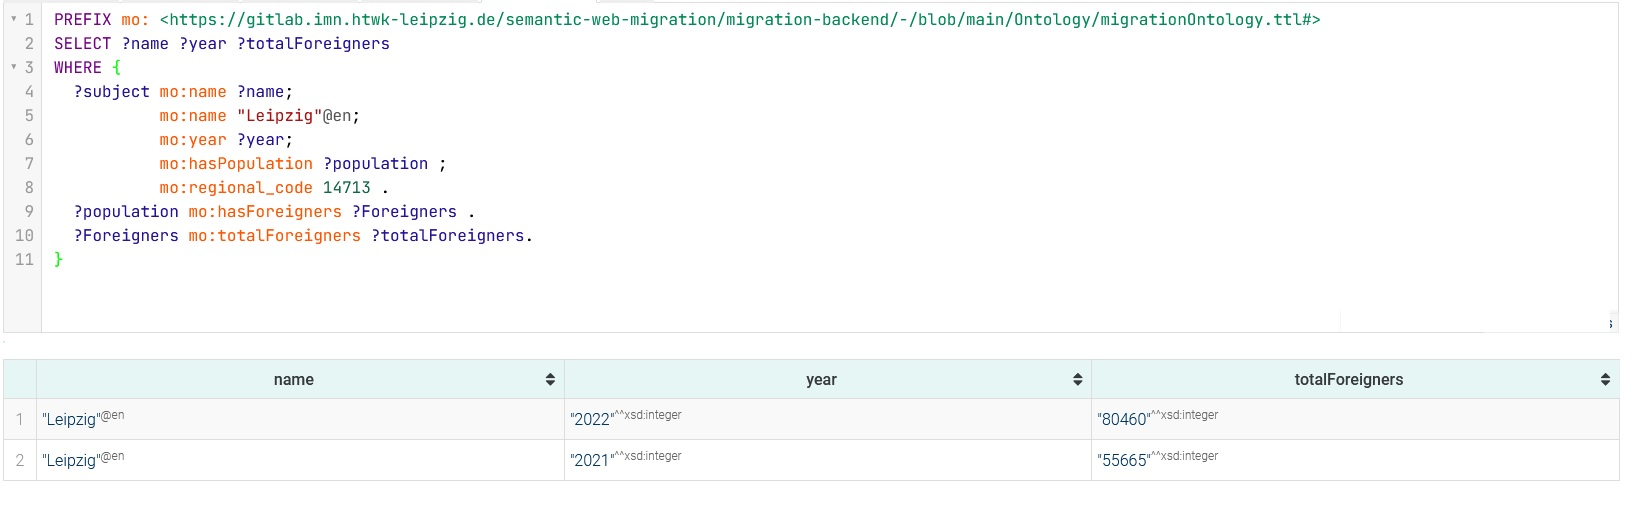
\includegraphics[width=1\textwidth]{Frage6.jpg} \\
    \item Wie viele Ausländer leben schon länger als 25 Jahre in Deutschland? \\ \\
    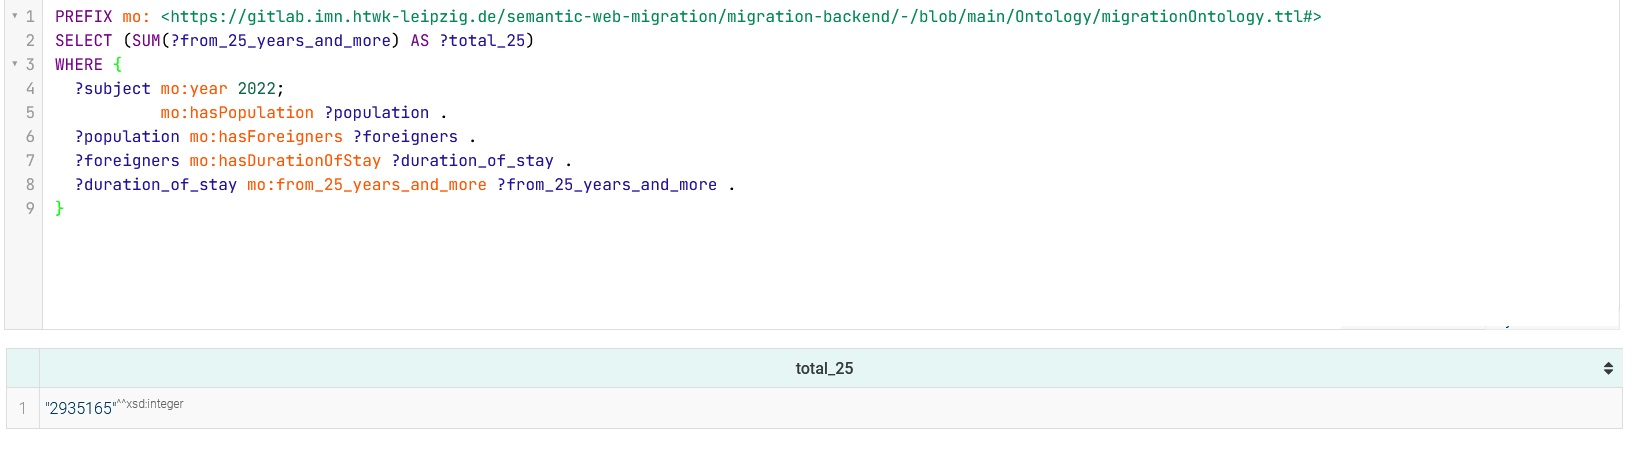
\includegraphics[width=1\textwidth]{Frage7.jpg} \\
\end{enumerate}

\section{Ergebnisse und Bedeutung}
Die vorliegende Forschungsarbeit hat eine wegweisende Semantic Web Anwendung zur Bevölkerungsdatenanalyse in deutschen Städten entwickelt. Die Verschmelzung von semantischer Modellierung und Datenanalyse erlaubte profunde Einblicke in Bevölkerungsstruktur, Migrationstrends und Demografie. Dieser Ansatz übertraf konventionelle statistische Methoden. Die eigens entwickelte Ontologie bildete das Grundgerüst, wobei durch Kompetenzfragen passende Klassen, Eigenschaften und Beziehungen definiert wurden. Der WebVOWL Editor erleichterte die Gestaltung komplexer Zusammenhänge visuell. Schritte wie Datenerfassung, Tripelgenerierung und Graphdatenbankintegration ermöglichten gezielte SPARQL-Abfragen.
\\ \\
Die Ergebnisse waren beeindruckend von Ausländeranteilen bis zu Asylsuchenden konnten relevante Daten gewonnen werden. Die Arbeit stellt nicht nur Antworten auf Forschungsfragen bereit, sondern auch wertvolle Erkenntnisse für soziale Dienste, Stadtplanung und Politik. Zusammenfassend eröffnet die Studie nicht nur eine effiziente Semantic Web-Anwendung zur \newline Bevölkerungsdatenanalyse, sondern zeigt auch neue Wege, wie das Semantic Web zur besseren Interpretation komplexer sozialer Phänomene genutzt werden kann. Die Verbindung von semantischer Modellierung, Datenanalyse und SPARQL-Abfragen verleiht der Auswertung von Bevölkerungsdaten eine präzisere und tiefgreifendere Bedeutung, mit Potenzial für vielfältige Anwendungen in Forschung und gesellschaftlicher Gestaltung.

\end{document}
